\documentclass[12pt,titlepage]{article}

\setlength{\oddsidemargin}{0in}
\setlength{\evensidemargin}{0in}
\setlength{\textwidth}{6.5in}
%
\setlength{\textheight}{9in}
\setlength{\topmargin}{0in}
\setlength{\headsep}{0in}
\setlength{\topskip}{0in}
\setlength{\headheight}{0in}

\usepackage{graphicx}
\usepackage{times}
\usepackage[plainpages=false, colorlinks=true, anchorcolor=blue, linkcolor=blue, citecolor=blue, bookmarks=false, urlcolor=blue]
{hyperref}
\usepackage[square,comma,authoryear]{natbib}


\title{DOE Office of Science INCITE Project:\\
{\it Extreme-scale Simulation of Supernovae and Magnetars from Realistic Progenitors}\\
2018 End-Of-Year Report}

\author{Principal Investigator:\\Sean M. Couch\\
  Michigan State University \vspace{0.1in}\\
  Co-Investigators: \\
  Andrew Christlieb (Michigan State University) \\
  Evan O'Connor (Stockholm University)\\
  Kuo-Chuan Pan (National Tsinghua University) \\
  Luke Roberts (Michigan State University) \\
  MacKenzie Warren (Michigan State University) \\
}

\date{January 1, 2019}


\begin{document}


\maketitle


%%%%%%%%%%%%%%%%%%%%%%%%%%%%%%%%%
\section{Project Usage}

%%%%%%%%%%%%%%%%%%%


\begin{figure}
  \begin{tabular}{cc}
    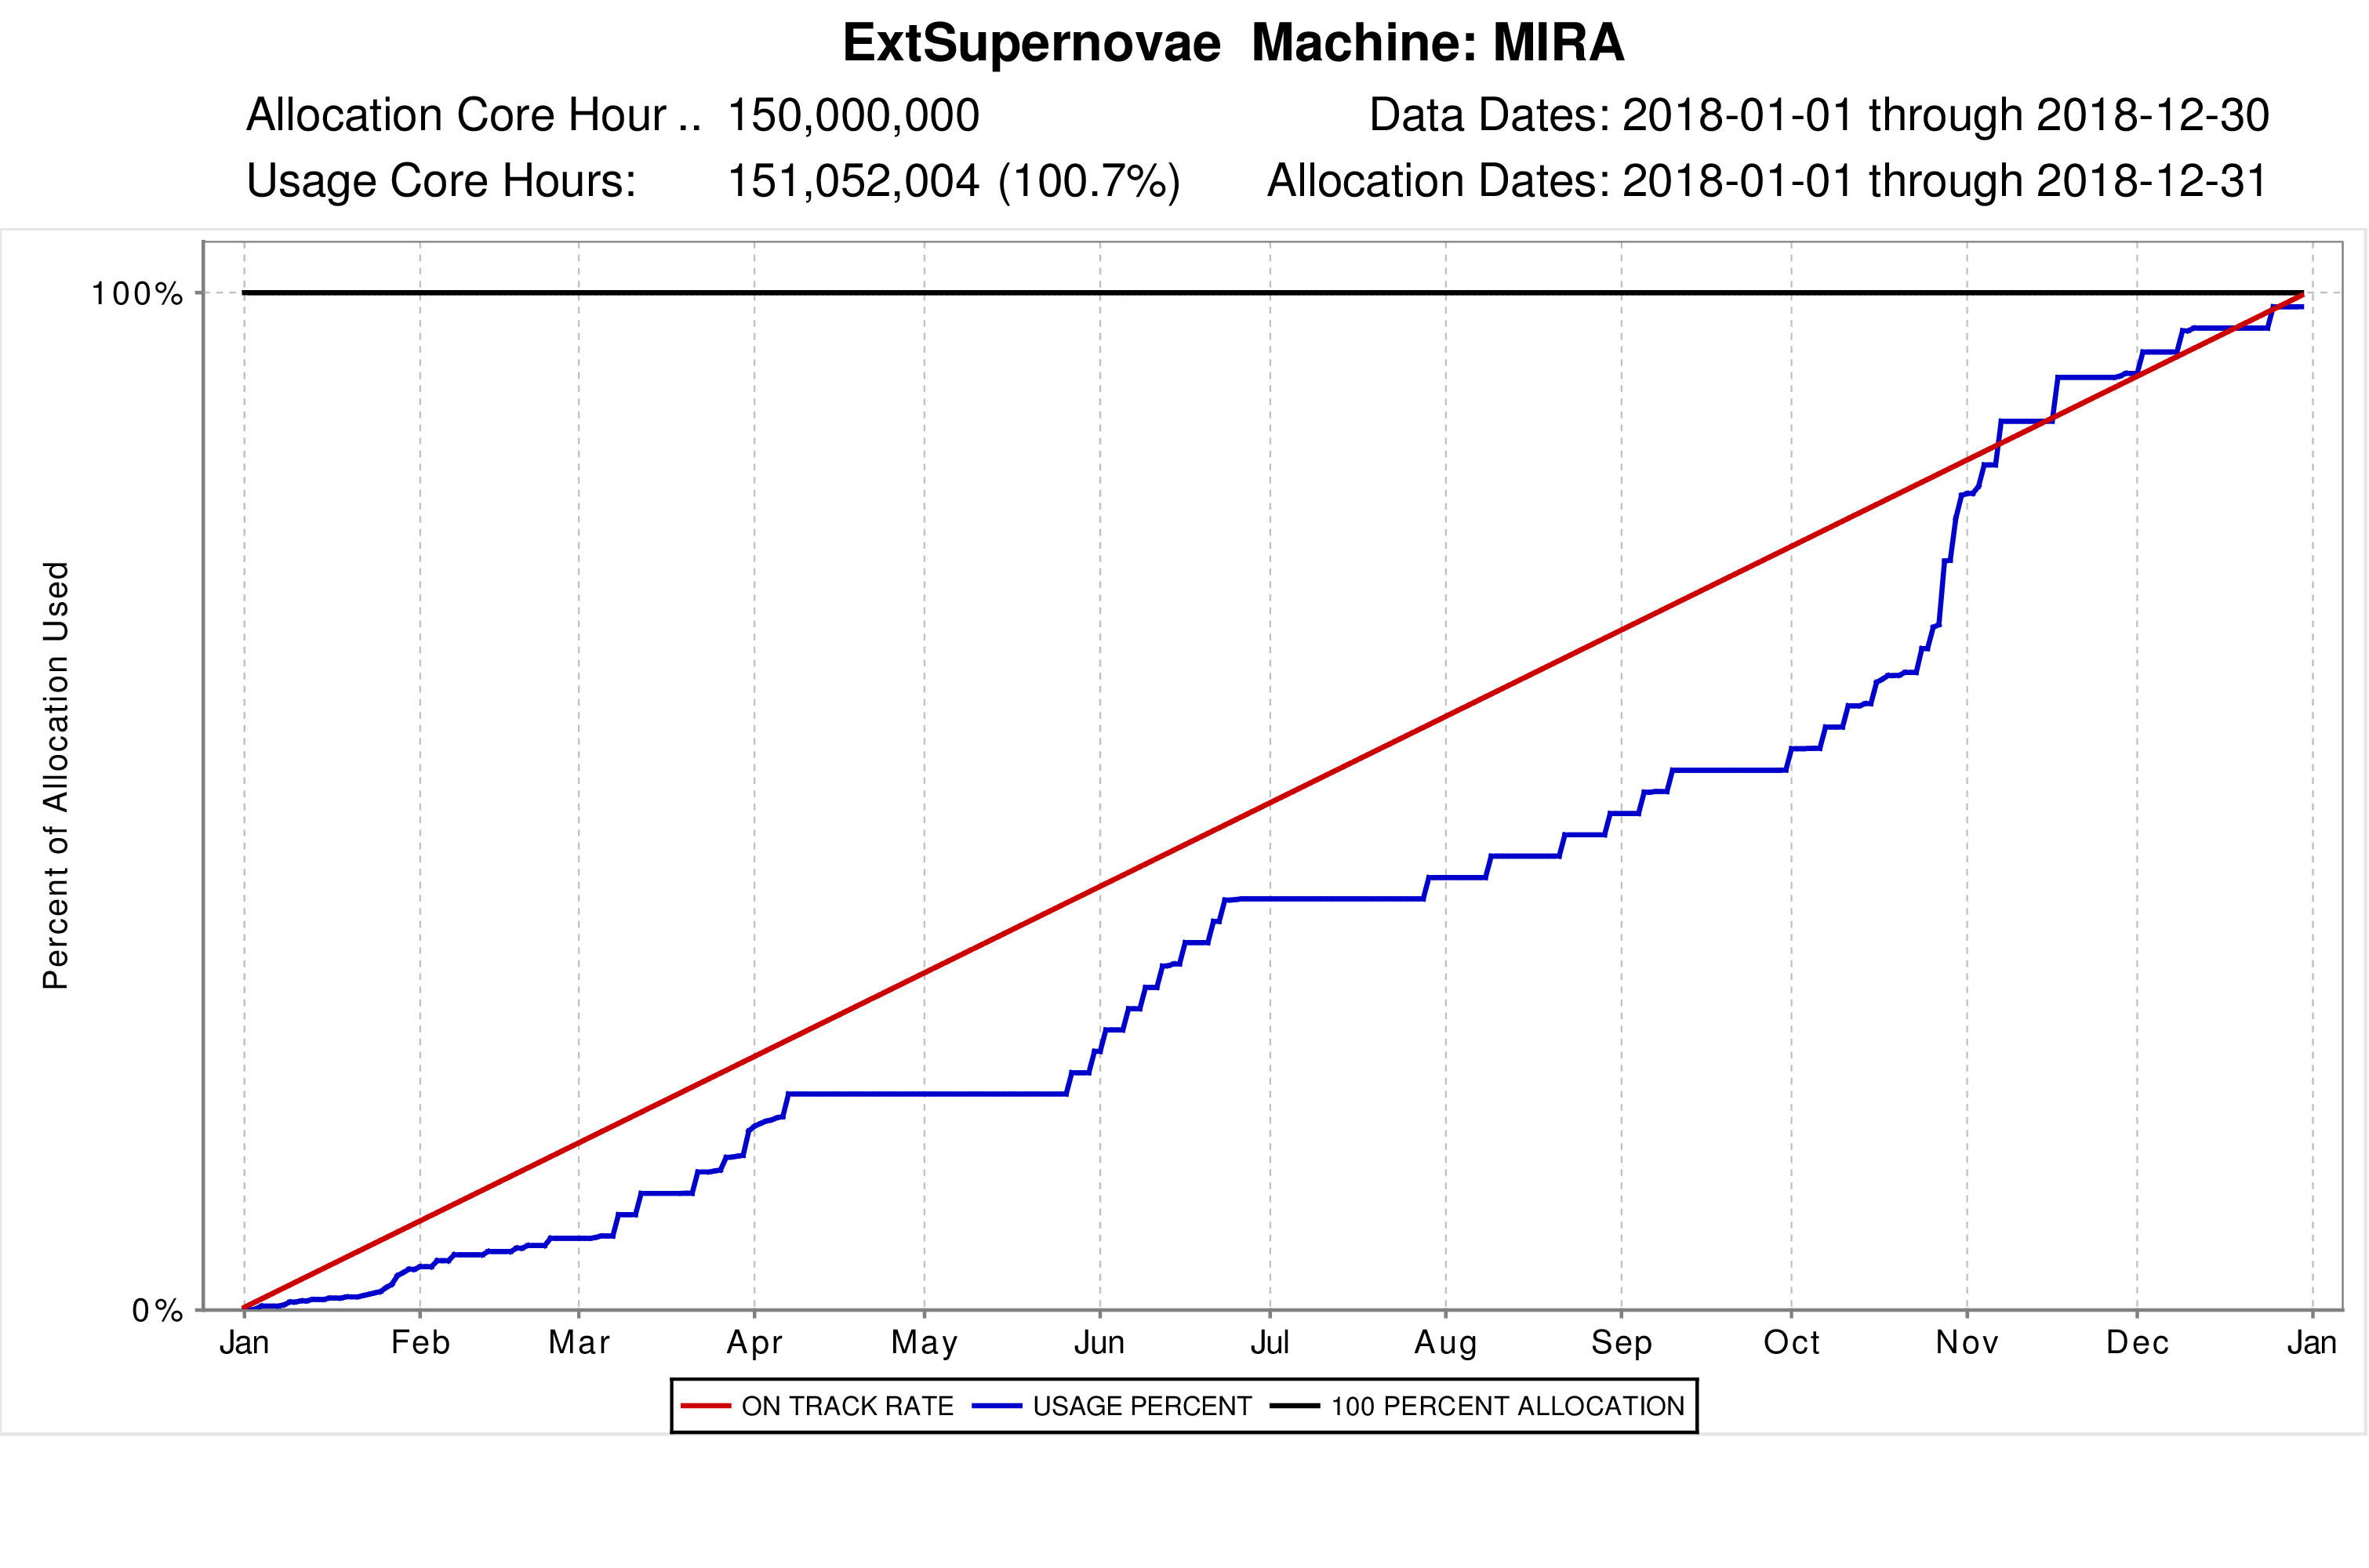
\includegraphics[width=3.25in]{on_track_graph_mira.png}
    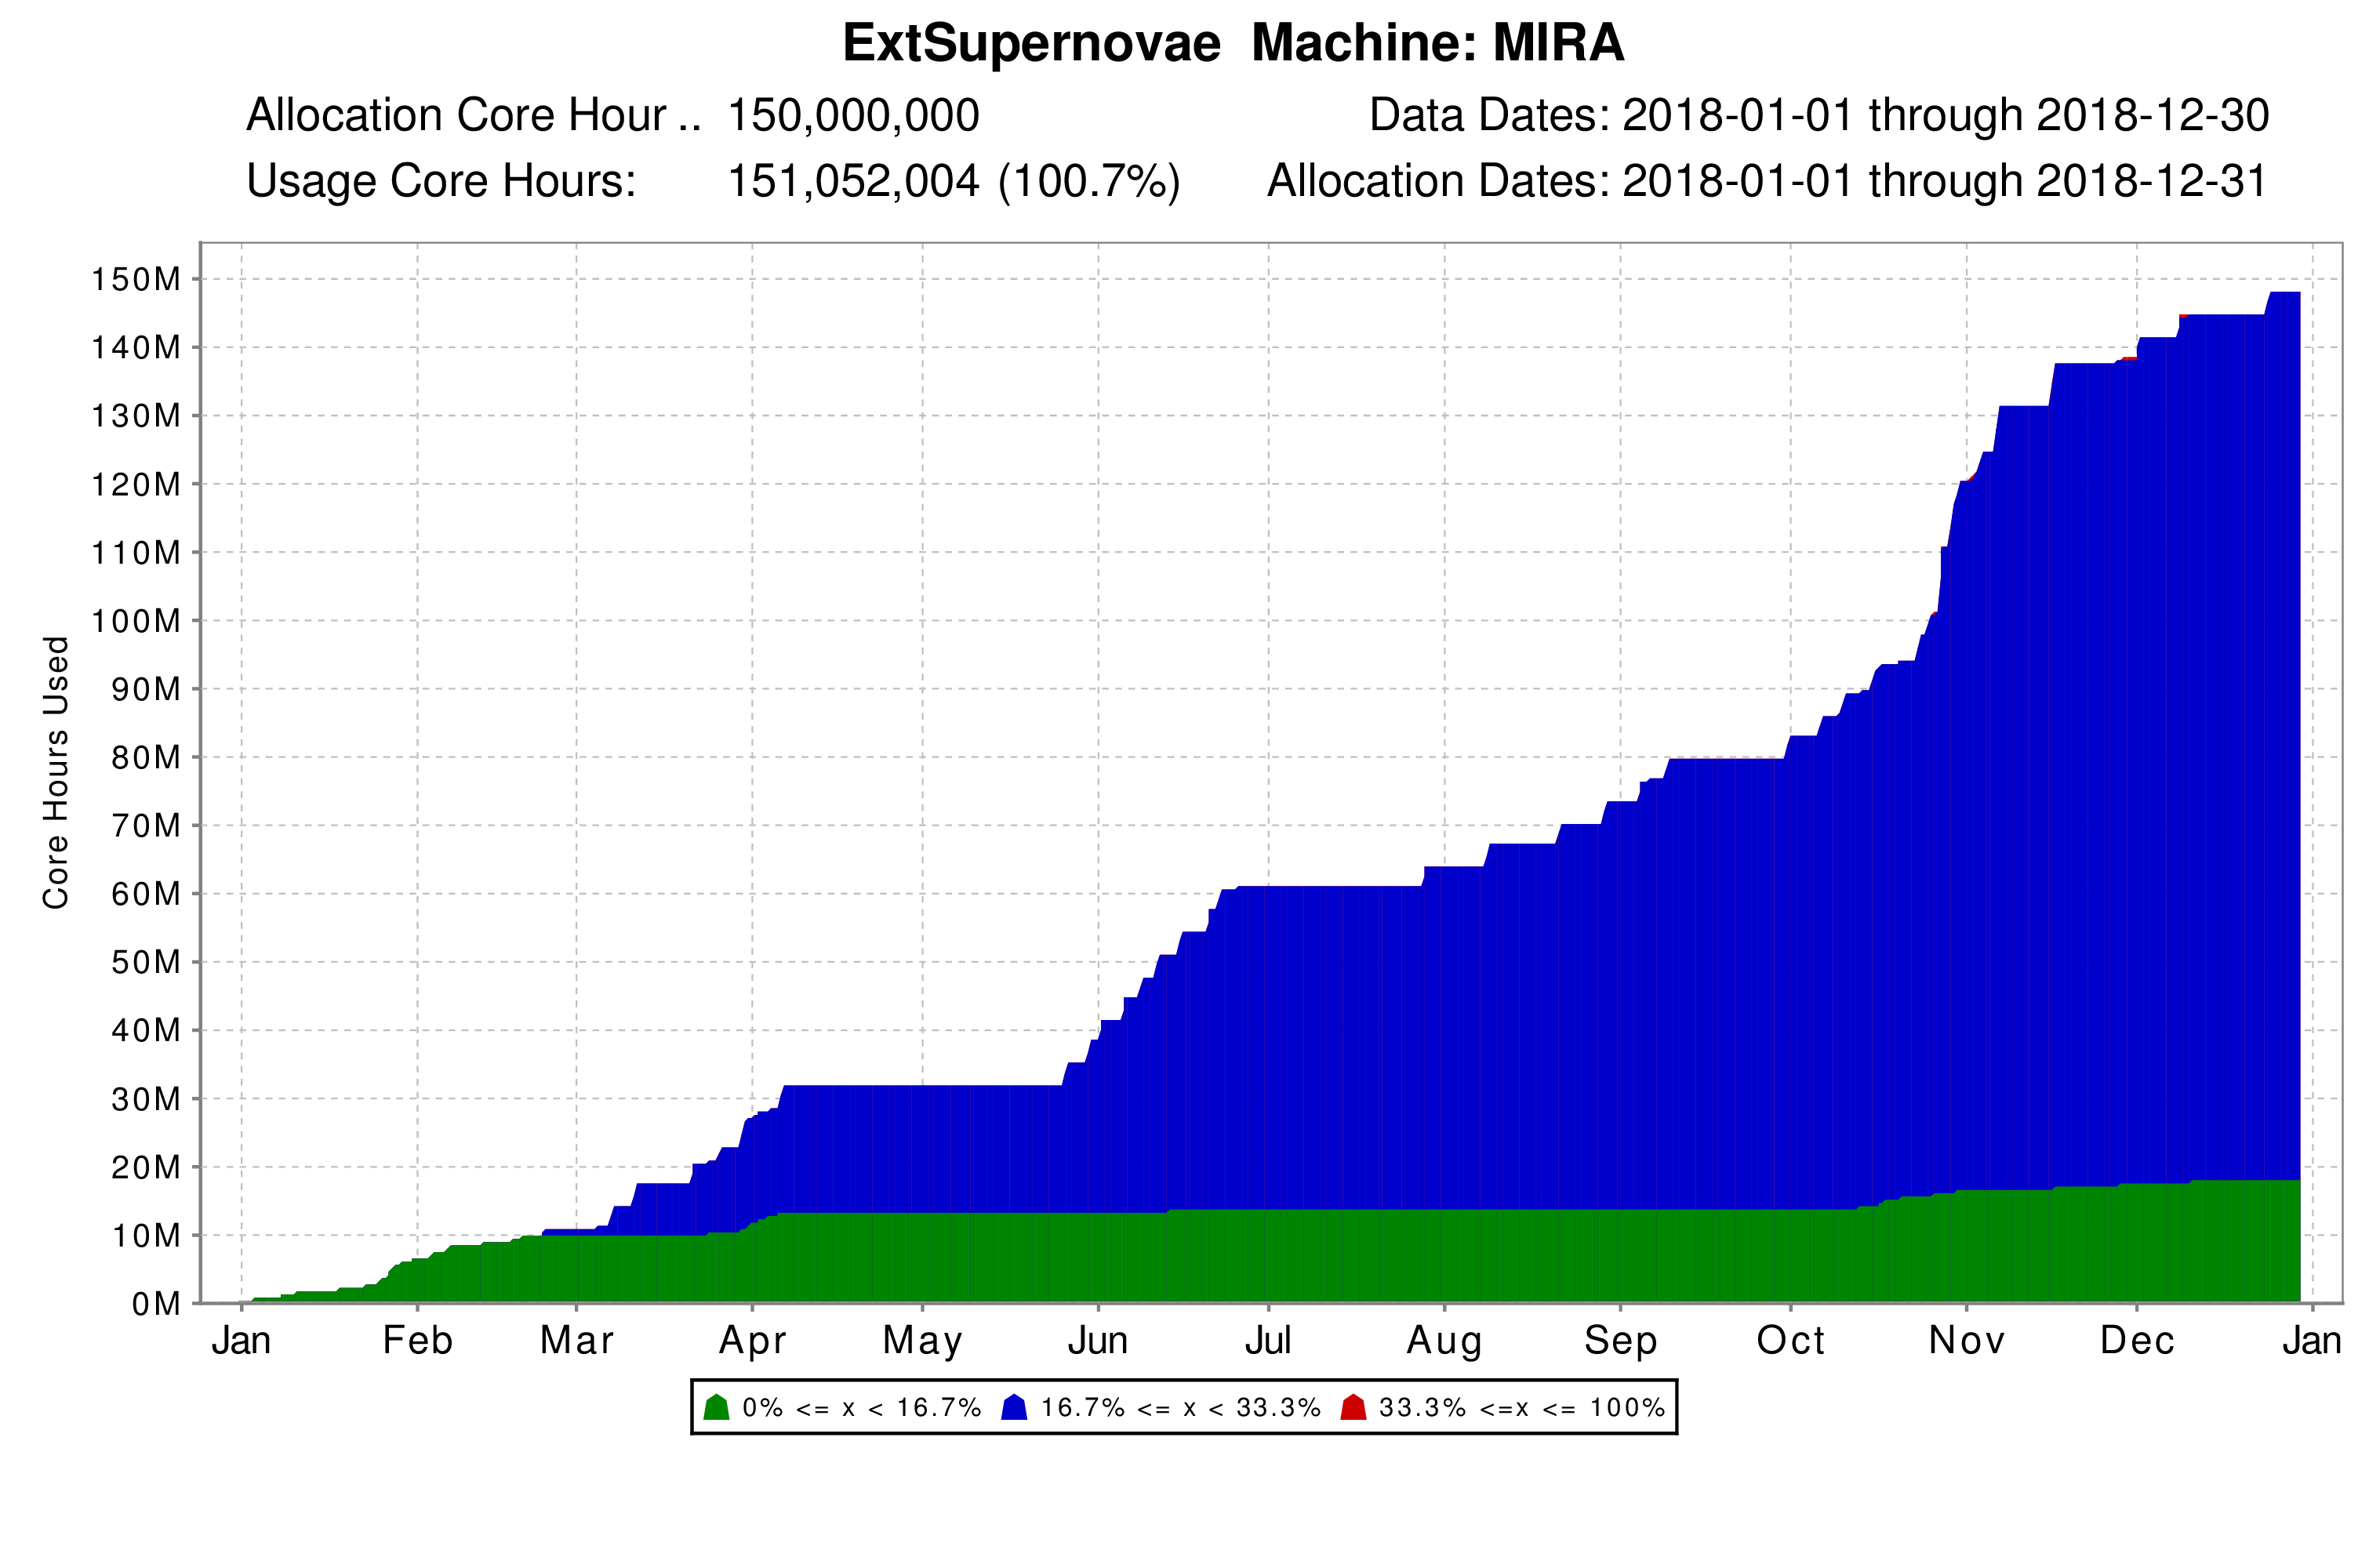
\includegraphics[width=3.25in]{categorized_hours_graph_mira.png} \\
    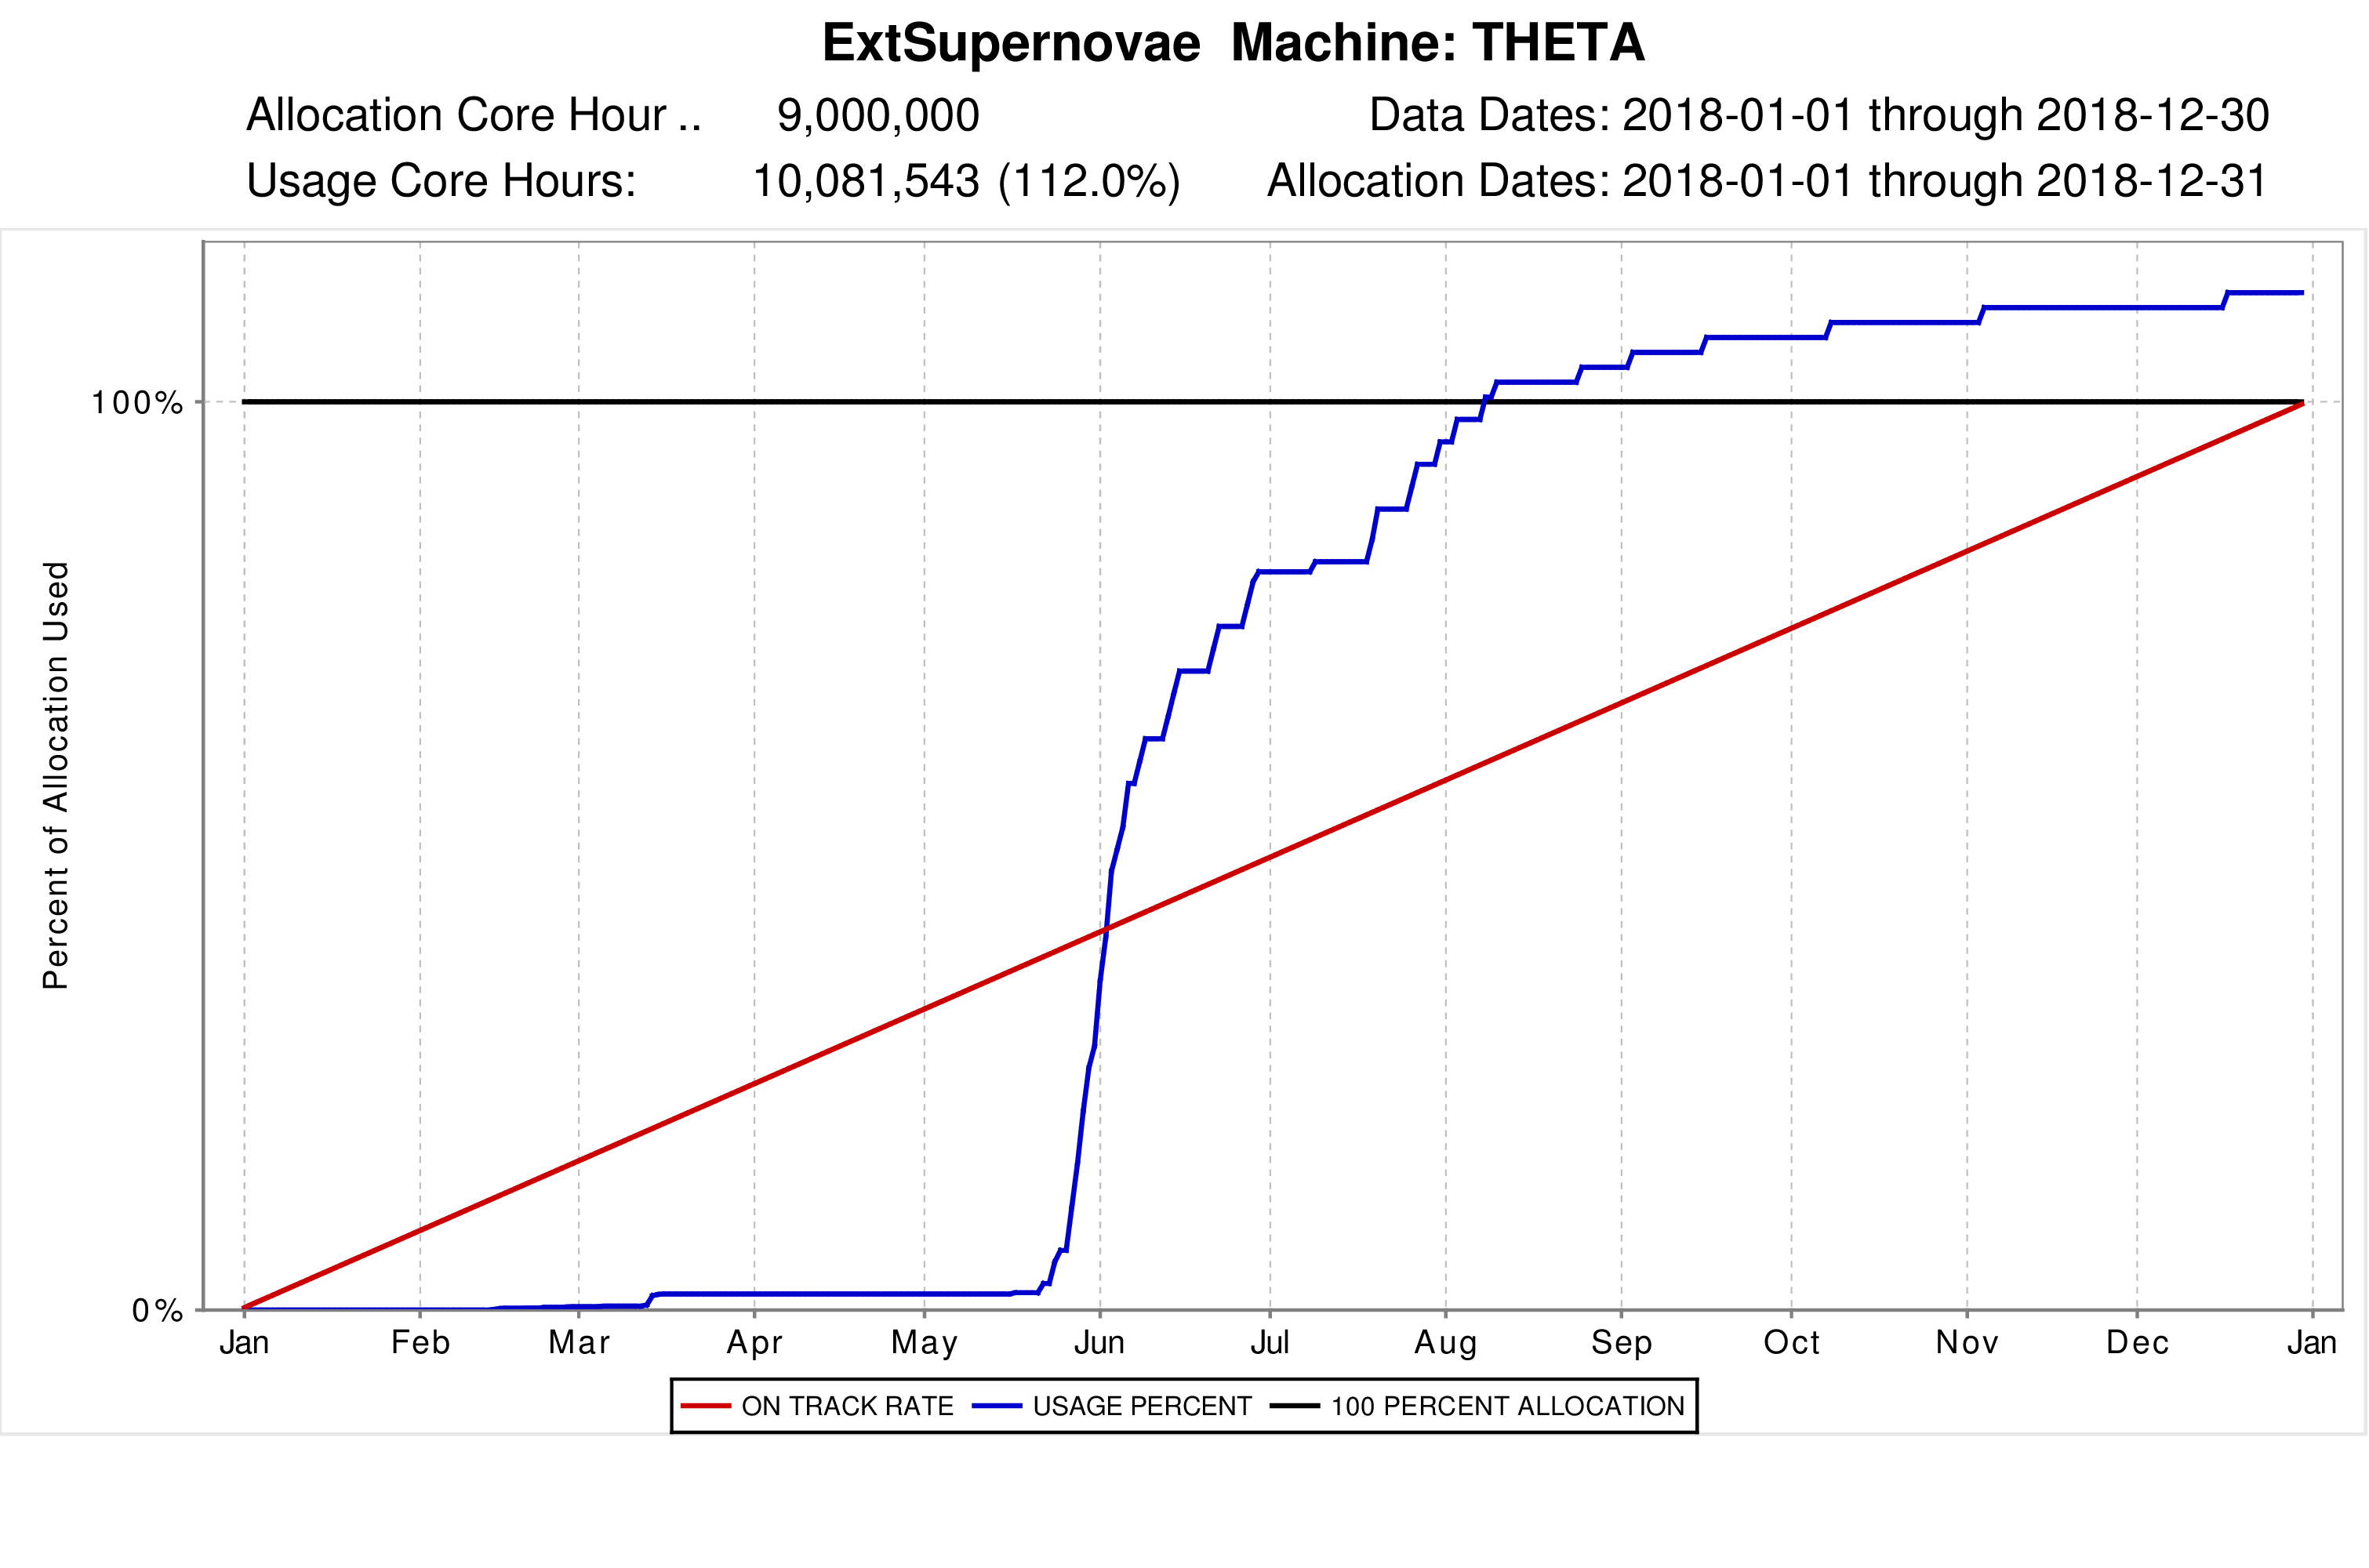
\includegraphics[width=3.25in]{on_track_graph}
    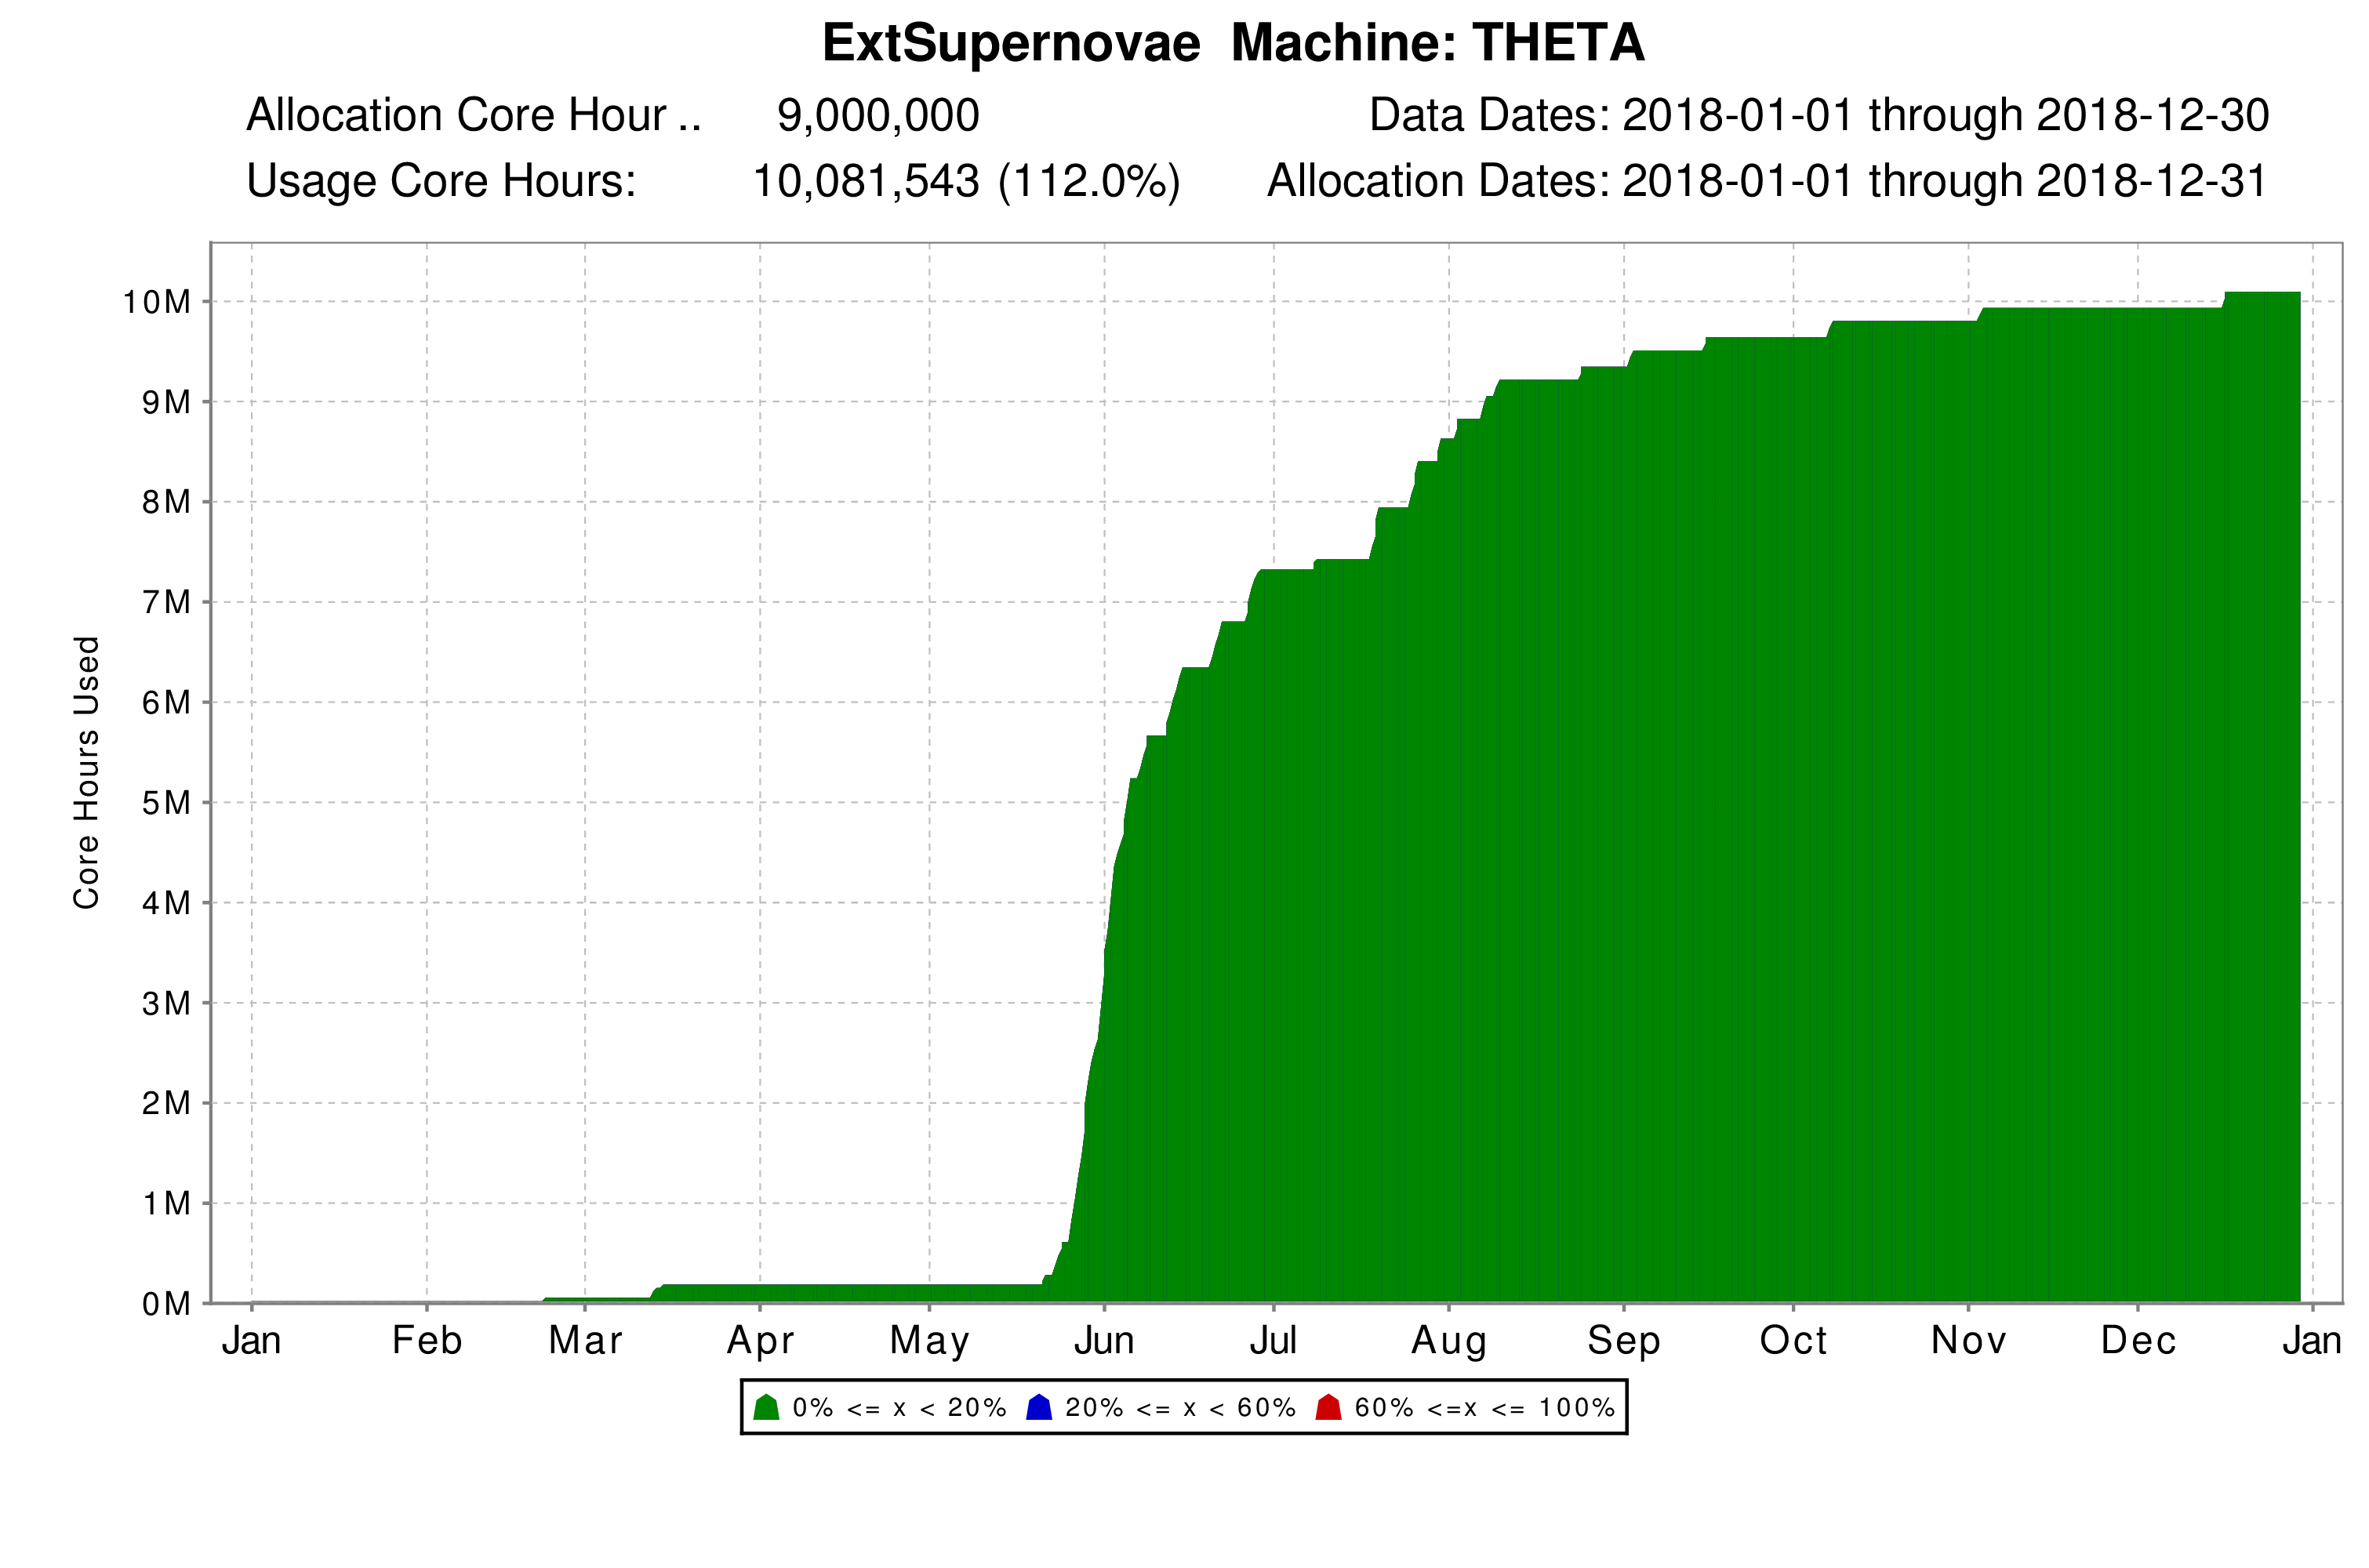
\includegraphics[width=3.25in]{categorized_hours_graph} 
  \end{tabular}
  \caption{Allocation usage.}
  \label{fig:usage}
\end{figure}

In 2018, we expended 151M core-hours on Mira, 101\% of our 2018 allocation (see Figure \ref{fig:usage}).
The vast majority of our usage on Mira was at the capability scale.
We expended 10.1M core-hours on Theta, 112\% of our 2018 allocation. 
We largely achieved our planned goals for simulations on both Mira and Theta. 
In 2019, some of these runs will be continued to later physical times.


%%%%%%%%%%%%%%%%%%%%%%%%%%%%%%%%%
\section{Report on Project Milestones}
%%%%%%%%%%%%%%%%%%%

Our milestones for Year 1, and corresponding progress, were:
\begin{enumerate}
  \item {\it 3D simulations of magnetorotational core-collapse supernovae} -- These simulations  progressed sufficiently that we are able to assess the impact of including rotation and magnetic fields. These simulations largely met our original scientific goals for 2018, though we plan to extend them to slightly later times in 2019 (as planned in our renewal). The simulations on Theta involved rapidly-rotating initial conditions and have moved very quickly, thanks to our greater computational efficiency on Theta and higher queue throughput.
  \item {\it 3D simulations of iron core collapse in massive stars} -- We completed one 3D octant simulation during Q4. This will serve as the basis for new models in 2019, as well as a paper that we are preparing for publication now.
  \item {\it High-resolution simulations of magnetorotational turbulence} -- This simulation consumed a significant portion of our allocation in Q4 and will provide a valuable resolution study when compared against our other results.
  \item {\it Develop SIMpliPy workflow tool} -- We mainly developed tools for post-processing analysis and visualization. 
  \item {\it Implement marching cubes for EOS and opacities} -- We have implemented other optimizations to the EOS and opacity table routines (primarily array re-ordering in the kernels) that has dramatically sped up this part of our simulations. So much so, it is not a significant fraction of runtime. Further optimization is on hold now.
\end{enumerate}



%%%%%%%%%%%%%%%%%%%%%%%%%%%%%%%%%
\section{Project Productivity}
%%%%%%%%%%%%%%%%%%%

\subsection{Primary}

\noindent {\bf Publications}
\begin{itemize}
  \item \href{https://ui.adsabs.harvard.edu/#abs/2018MNRAS.481.3293R/abstract}{``The antesonic condition for the explosion of core-collapse supernovae - I. Spherically symmetric polytropic models: stability and wind emergence''}, Raives, M. J., Couch, S. M., Greco, J. P., Pejcha, O., Thompson, T. A. 2018, {\itshape Monthly Notices of the Royal Astronomical Society}, 481, 3293 (3 citations)

  \item \href{https://ui.adsabs.harvard.edu/#abs/2018ApJ...865...81O/abstract}{``Exploring Fundamentally Three-dimensional Phenomena in High-fidelity Simulations of Core-collapse Supernovae''}, O'Connor, E. P., Couch, S. M. 2018, {\itshape The Astrophysical Journal}, 865, 81 (18 citations)
  
  \item \href{https://ui.adsabs.harvard.edu/#abs/2018JPhG...45j4001O/abstract}{``Global comparison of core-collapse supernova simulations in spherical symmetry''}, O'Connor, E., Bollig, R., Burrows, A., et al.\ 2018, {\itshape Journal of Physics G Nuclear Physics}, 45, 104001 (9 citations)
  
  \item \href{https://ui.adsabs.harvard.edu/#abs/2018JPhG...45e3003R/abstract}{``Turbulence in core-collapse supernovae''}, Radice, D., Abdikamalov, E., Ott, C. D., M\"osta, P., Couch, S. M., Roberts, L. F. 2018, {\itshape Journal of Physics G Nuclear Physics}, 45, 053003 (13 citations)
  
  \item \href{https://ui.adsabs.harvard.edu/#abs/2018ApJ...857...13P/abstract}{``Equation of State Dependent Dynamics and Multi-messenger Signals from Stellar-mass Black Hole Formation''}, Pan, K., Liebendörfer, M., Couch, S. M., Thielemann, F. 2018, {\itshape The Astrophysical Journal}, 857, 13 (15 citations)
  
  \item \href{https://ui.adsabs.harvard.edu/#abs/2018ApJ...854...63O/abstract}{``Two-dimensional Core-collapse Supernova Explosions Aided by General Relativity with Multidimensional Neutrino Transport''}, O'Connor, E. P., Couch, S. M. 2018, {\itshape The Astrophysical Journal}, 854, 63 (46 citations)
\end{itemize}

\noindent {\bf Presentations}

\begin{itemize}
  \item ``Understanding Massive Stellar Death: Predictive Simulation of Core-collapse Supernovae,'' S.M. Couch, Oskar Klein Centre Colloquium, Stockholm University, Stockholm, Sweden, October 2018
  \item ``Understanding Massive Stellar Death: Predictive Simulation of Core-collapse Supernovae,'' S.M. Couch, Physics Colloquium, Notre Dame University, Notre Dame, IN, October 2018
  \item ``Understanding Massive Stellar Death: Predictive Simulation of Core-collapse Supernovae,'' S.M. Couch, CCAPP Seminar, Ohio State University, Columbus, OH, April 2018
  \item ``Understanding Massive Stellar Death: Predictive Simulation of Core-collapse Supernovae,'' S.M. Couch, Physics and Astronomy Colloquium, Louisiana State University, Baton Rouge, LA, March 2018
  \item ``Understanding Massive Stellar Death: Predictive Simulation of Core-collapse Supernovae,'' S.M. Couch, Physics and Astronomy Colloquium, University of Alabama, Tuscaloosa, AL, February 2018
\end{itemize}

\subsubsection{Secondary}

\begin{itemize}
  \item Co-I and postdoc Kuo-Chuan Pan started a tenure-track faculty position at National Tsing Hua University in Taiwan.
  \item Co-I and postdoc MacKenzie Warren won a prestigious NSF Postdoctoral Fellowship.
\end{itemize}

\section{Center Feedback}

Our catalyst, Adrian Pope, has been extremely helpful.
We have been experience occasional, seemingly random, I/O errors when reading large checkpoint files at startup.
He helped us debug this and by the end of the Year we were no longer seeing this error.


\section{Code Description and Characterization}

\texttt{FLASH} is a highly capable, fully modular, extensible,
community code that is widely used in astrophysics, cosmology, fluid
dynamics, and plasma physics, and other fields.  The capabilities of
the FLASH code include adaptive mesh refinement (AMR), several
self-gravity solvers, an advection-diffusion-reaction (ADR) flame
model, an accurate and detailed treatment of nuclear burning, and a
sophisticated two-moment neutrino transport scheme based on an
explicit hyperbolic solver.  The neutrino interactions are included
through the open-source neutrino interaction library
\texttt{NuLib}. We have enhanced the
performance of the two-moment neutrino transport scheme significantly
as well as upgraded the transport to now include full velocity and
gravitational red-shift dependence in the evolution equations.

\texttt{FLASH} is written in modern Fortran, with some utility
functions written in C, and a build system written in Python.  It
requires MPI library support, and either HDF5 or P-NetCDF for I/O.
Additional mathematical software, such as \texttt{Hypre}, may be
required to configure \texttt{FLASH} for particular simulations.

Algorithm classes used within \texttt{FLASH} include Sparse Linear
Algebra solvers, FFT, active and passive particles, structured grids,
and AMR.



\end{document}
